% ============================================================
%  Chapter 3: System Architecture (Enhanced)
%  Includes: OpenFaaS, Two-Phase RL, 5-Layer Model,
%  TikZ diagrams, pgfplots, booktabs tables, code listings
% ============================================================
\chapter{System Architecture}
\label{chap:architecture}

% ──────────────────────────────────────────────────────────────────────────────
\section{Overview}
% ──────────────────────────────────────────────────────────────────────────────

This chapter presents the complete architecture of the \textbf{Serverless Spark
Framework for Real-Time IoT Applications}. The framework integrates five distinct
functional layers:

\begin{enumerate}
  \item \textbf{IoT Edge Layer} --- synthetic sensor generation with burst-prediction.
  \item \textbf{Ingestion Layer} --- dual-lane MQTT (control) and Apache Kafka (data).
  \item \textbf{Optimization Engine} --- Two-Phase Hierarchical RL (TD3 + PPO).
  \item \textbf{OpenFaaS Serverless Orchestration} --- event-driven RL function deployment.
  \item \textbf{Spark Execution Layer} --- dynamic distributed processing.
\end{enumerate}

Unlike the original single-layer Spark framework, this architecture incorporates a
\textbf{Two-Phase Reinforcement Learning} system and an \textbf{OpenFaaS serverless
function} as the central decision engine. This design enables proactive, cost-aware,
and latency-sensitive resource scaling --- a critical advantage over the static
executor configurations used in conventional deployments.

All modules are fully containerised via Docker Compose, ensuring reproducibility,
portability, and isolation across development and production environments.


% ──────────────────────────────────────────────────────────────────────────────
\section{Technology Stack}
% ──────────────────────────────────────────────────────────────────────────────

Table~\ref{tab:tech_stack} lists the complete software stack employed in this framework,
updated to include the RL and serverless components.

\begin{table}[H]
\centering
\caption{Complete Technology Stack}
\label{tab:tech_stack}
\begin{adjustbox}{max width=\textwidth}
\begin{tabular}{|p{3.2cm}|p{4cm}|p{6.5cm}|}
\hline
\textbf{Component}       & \textbf{Technology}              & \textbf{Purpose / Justification} \\ \hline
Language                 & Python 3.11                      & Unified language across all modules. \\ \hline
Containerisation         & Docker 24 + Compose              & Reproducible multi-service deployment. \\ \hline
IoT Protocol             & MQTT (Mosquitto 2.0)             & Lightweight IoT control-plane protocol. \\ \hline
Streaming Platform       & Apache Kafka 3.6 + ZooKeeper 3.8 & Durable, partitioned data-plane ingestion. \\ \hline
Processing Engine        & Apache Spark 3.5 (Structured Streaming) & Distributed micro-batch analytics. \\ \hline
RL Framework             & Stable-Baselines3 (PPO + TD3)    & Two-Phase Hierarchical RL optimizer. \\ \hline
Serverless Orchestrator  & OpenFaaS (python3-http)          & Event-driven, scale-to-zero RL inference. \\ \hline
Edge Burst Predictor     & Pattern Feature Extractor (7-dim)& Cold-start mitigation via pre-warming. \\ \hline
Cache / State Store      & Redis 7.2                        & Fast in-memory metrics buffer. \\ \hline
Monitoring               & Docker Stats, Spark UI, Kafka CLI & Runtime health and throughput visibility. \\ \hline
\end{tabular}
\end{adjustbox}
\end{table}


% ──────────────────────────────────────────────────────────────────────────────
\section{Five-Layer Architectural Model}
\label{sec:five_layer}
% ──────────────────────────────────────────────────────────────────────────────

Figure~\ref{fig:five_layer_arch} presents the complete five-layer architecture with all
cross-layer data flows, feedback loops, and the OpenFaaS integration.

\begin{figure}[H]
\centering
\begin{tikzpicture}[
    layer/.style={rectangle, draw, rounded corners=5pt, minimum width=11.5cm,
                  minimum height=1.0cm, font=\footnotesize, align=center},
    arr/.style={-{Stealth[length=2.5mm]}, thick},
    scale=0.80, transform shape
]
\definecolor{cl1}{RGB}{96,165,250}
\definecolor{cl2}{RGB}{120,80,180}
\definecolor{cl3}{RGB}{52,211,153}
\definecolor{cl4}{RGB}{255,165,0}
\definecolor{cl5}{RGB}{230,76,60}

\node[layer, fill=cl1!20, draw=cl1] (L1) at (0, 5.0)
    {\textbf{Layer 1 — IoT Edge:} Smart City / Healthcare / Industrial Sensors
     + Edge Gateway (Burst Prediction $P_{burst}$)};

\node[layer, fill=cl2!15, draw=cl2] (L2) at (0, 3.6)
    {\textbf{Layer 2 — Ingestion:}
     Kafka (bulk data) $\parallel$ MQTT (control signals) — Dual-Lane Pipeline};

\node[layer, fill=cl3!20, draw=cl3, minimum height=1.4cm] (L3) at (0, 1.9)
    {\textbf{Layer 3 — RL Optimization Engine}\\
     TD3 Meta-Controller (Phase 2, every episode)
     $\longrightarrow$ PPO Resource Agent (Phase 1, every 5 s)};

\node[layer, fill=cl4!20, draw=cl4] (L4) at (0, 0.5)
    {\textbf{Layer 4 — OpenFaaS Serverless:}
     \texttt{rl-scaling-function} — HTTP endpoint, scale-to-zero};

\node[layer, fill=cl5!15, draw=cl5] (L5) at (0,-0.9)
    {\textbf{Layer 5 — Spark Execution:}
     Dynamic Executors (0--50) + Redis HOT / NVMe WARM / S3 COLD};

% Forward arrows
\draw[arr, cl1] (L1) -- (L2);
\draw[arr, cl2] (L2) -- (L3);
\draw[arr, cl3] (L3) -- (L4);
\draw[arr, cl4] (L4) -- (L5);

% Feedback: Spark -> RL
\draw[arr, cl5, dashed] (L5.east) to[bend left=55]
    node[right, font=\scriptsize]{reward feedback} (L3.east);

% Feedback: Edge -> RL
\draw[arr, cl1, dashed] (L1.west) to[bend right=55]
    node[left, font=\scriptsize]{burst signal} (L3.west);
\end{tikzpicture}
\caption{Final five-layer architecture of the Serverless Spark IoT Framework including
the Two-Phase RL Optimization Engine and OpenFaaS serverless orchestration.}
\label{fig:five_layer_arch}
\end{figure}

\noindent Each layer is independently deployable, enabling hybrid edge--cloud configurations.
The dual feedback loops (reward from Spark and burst signals from the edge gateway)
are essential for proactive, closed-loop resource management.


% ──────────────────────────────────────────────────────────────────────────────
\section{End-to-End Data Flow}
\label{sec:e2e_flow}
% ──────────────────────────────────────────────────────────────────────────────

Figure~\ref{fig:e2e_flow} shows the detailed end-to-end data and control flow across
all five layers, distinguishing between the high-throughput data path (solid arrows)
and the low-latency control path (dashed arrows).

\begin{figure}[H]
\centering
\begin{tikzpicture}[
    box/.style={rectangle, draw, rounded corners=4pt, minimum height=0.85cm,
                minimum width=1.8cm, font=\scriptsize, align=center},
    arr/.style={-{Stealth[length=2.5mm]}, thick},
]
%% TOP ROW — data path
\node[box, fill=blue!15]     (iot)   at (0,0)     {IoT\\Sensors};
\node[box, fill=blue!15]     (edge)  at (2.6,0)   {Edge\\Gateway};
\node[box, fill=purple!15]   (kafka) at (5.2,0)   {Apache\\Kafka};
\node[box, fill=red!10]      (spark) at (7.8,0)   {Spark\\Executors};

%% BOTTOM ROW — RL control path
\node[box, fill=green!12]    (meta)  at (2.6,-2.6){TD3\\Meta-Ctrl};
\node[box, fill=green!20]    (ppo)   at (5.2,-2.6){PPO\\Agent};
\node[box, fill=orange!20]   (faas)  at (7.8,-2.6){OpenFaaS\\Function};

%% Data path arrows
\draw[arr] (iot.east)   -- (edge.west);
\draw[arr] (edge.east)  -- (kafka.west);
% Kafka streams data to Spark over the top
\draw[arr] (kafka.north) -- ++(0,0.6)
    -- node[above, font=\tiny]{data stream} ++(2.6,0)
    -- (spark.north);

%% Kafka -> RL metrics
\draw[arr] (kafka.south) -- ++(0,-0.55) -|
    node[left, font=\tiny, pos=0.65]{metrics} (meta.north);
% Meta -> PPO weights
\draw[arr, purple] (meta.east) --
    node[above, font=\tiny]{$\alpha,\beta,\gamma$} (ppo.west);
% Kafka features to PPO
\draw[arr, dashed, blue!60] (kafka.south) -- ++(0,-0.55) -|
    node[right, font=\tiny, pos=0.5]{features} (ppo.north);

%% Edge burst -> PPO
\draw[arr, dashed, blue] (edge.south) -- ++(0,-0.8) -|
    node[below, font=\tiny, near start]{burst signal} (ppo.north);

%% RL -> OpenFaaS -> Spark
\draw[arr, green!60!black] (ppo.east) --
    node[above, font=\tiny]{decision} (faas.west);
\draw[arr, orange!80!black] (faas.north) -- ++(0,0.55) -|
    node[right, font=\tiny, pos=0.3]{scale cmd} (spark.south);

%% Reward feedback: Spark -> Meta
\draw[arr, dashed, red!60]
    (spark.east) -- ++(0.6,0)
    -- ++(0,-3.55)
    -| node[below, font=\tiny, near start]{reward} (meta.south);
\end{tikzpicture}
\caption{End-to-end data and control flow. Solid arrows = data path $(\text{Kafka} \to \text{Spark})$.
Dashed arrows = RL feedback loops.}
\label{fig:e2e_flow}
\end{figure}

\noindent The control sequence proceeds as follows at runtime:
\begin{enumerate}
  \item IoT sensors emit telemetry every 2 s; the edge gateway computes a 7-feature
        burst-probability signature $P_{burst}$ and forwards it via MQTT.
  \item High-throughput data flows through Kafka topics; MQTT carries lightweight
        control signals to avoid data-plane congestion.
  \item The TD3 Meta-Controller observes episode-level SLA and cost health and updates
        $(\alpha, \beta, \gamma)$ weights for the PPO agent.
  \item The PPO agent selects a scaling action (\texttt{SCALE\_UP},
        \texttt{SCALE\_DOWN}, \texttt{MAINTAIN}, \texttt{PRE\_WARM}).
  \item The decision is sent as a JSON request to the OpenFaaS gateway.
  \item The \texttt{rl-scaling-function} returns the target executor count and the
        Spark Driver REST API applies the configuration.
  \item Step-level reward (latency, cost, throughput) flows back to PPO; episode-level
        statistics flow to TD3, closing both feedback loops.
\end{enumerate}


% ──────────────────────────────────────────────────────────────────────────────
\section{Containerised Runtime Environment}
\label{sec:containers}
% ──────────────────────────────────────────────────────────────────────────────

All services run inside Docker containers on a shared bridge network.
Table~\ref{tab:resource_usage} summarises average resource utilisation across all
services during a 24-hour continuous IoT workload trace.

\begin{table}[H]
\centering
\caption{Average Resource Utilisation During Continuous Operation}
\label{tab:resource_usage}
\begin{tabular}{lcccc}
\toprule
\textbf{Service}          & \textbf{CPU (\%)} & \textbf{Memory (MB)} &
  \textbf{Network In (KB/s)} & \textbf{Network Out (KB/s)} \\
\midrule
ZooKeeper                 & 0.3  & 65   & 2   & 2  \\
Kafka                     & 1.2  & 210  & 480 & 480 \\
Mosquitto (MQTT)          & 0.2  & 60   & 12  & 12  \\
Redis                     & 1.1  & 85   & 40  & 38  \\
Serverless Spark (master) & 2.8  & 588  & 210 & 195 \\
OpenFaaS Gateway          & 0.5  & 120  & 95  & 92  \\
RL Scaling Function       & 0.3  & 256  & 45  & 42  \\
\midrule
\textbf{Total}            & \textbf{6.4} & \textbf{1384} & -- & -- \\
\bottomrule
\end{tabular}
\end{table}

\noindent Total resource consumption remains well below 10\% CPU and 1.5 GB RAM,
confirming suitability for edge deployment on commodity hardware. The OpenFaaS
function contributes only 0.3\% CPU because it scales to zero between invocations
and is reloaded only when a new metrics payload arrives.

\subsection{Docker Compose Configuration}

\begin{lstlisting}[language=yaml, caption={Complete Docker Compose --- All Services
Including OpenFaaS and the RL Scaling Function}]
version: '3.9'

services:
  zookeeper:
    image: wurstmeister/zookeeper
    ports: ["2181:2181"]

  kafka:
    image: wurstmeister/kafka:2.13-2.8.1
    ports: ["9092:9092"]
    environment:
      KAFKA_ADVERTISED_HOST_NAME: kafka
      KAFKA_ZOOKEEPER_CONNECT:   zookeeper:2181
      KAFKA_CREATE_TOPICS: "iot-smartcity-raw:1:1,iot-healthcare-raw:1:1,iot-industrial-raw:1:1"
    depends_on: [zookeeper]

  mosquitto:
    image: eclipse-mosquitto:2
    ports: ["1883:1883", "9001:9001"]
    volumes: ["./mosquitto/mosquitto.conf:/mosquitto/config/mosquitto.conf"]

  redis:
    image: redis:7.2-alpine
    ports: ["6379:6379"]

  spark-master:
    image: bitnami/spark:3.5
    environment: [SPARK_MODE=master]
    ports: ["8080:8080", "7077:7077"]

  spark-worker:
    image: bitnami/spark:3.5
    environment:
      - SPARK_MODE=worker
      - SPARK_MASTER_URL=spark://spark-master:7077
    depends_on: [spark-master]

  openfaas-gateway:
    image: ghcr.io/openfaas/gateway:latest
    ports: ["8081:8080"]
    environment:
      - functions_provider_url=http://faasd:8081/
      - direct_functions=true

  rl-scaling-function:
    build: ./serverless/openfaas/rl-scaling-function
    image: rl-scaling-function:latest
    environment:
      - MODEL_PATH=/home/app/function/models/rl_optimizer
      - PREWARM_ENABLED=true
    labels:
      - "com.openfaas.scale.zero=true"
      - "com.openfaas.scale.zero-duration=5m"
\end{lstlisting}


% ──────────────────────────────────────────────────────────────────────────────
\section{Layer 1: IoT Edge — Data Generation}
\label{sec:layer1}
% ──────────────────────────────────────────────────────────────────────────────

Three independent generators reproduce realistic patterns for distinct IoT domains:

\begin{table}[H]
\centering
\caption{IoT Domain Generators and Their Metrics}
\label{tab:iot_domains}
\begin{tabular}{lll}
\toprule
\textbf{Domain}   & \textbf{Metrics Generated}                              & \textbf{Pattern}       \\
\midrule
Smart City        & Vehicle count, avg speed, AQI, parking occupancy        & Diurnal rush-hour cycle \\
Healthcare        & Heart rate, BP, SpO$_2$, ECG amplitude, alert flag       & Work-shift with spikes  \\
Industrial        & Temperature, vibration, power load, wear index          & Continuous with bursts  \\
\bottomrule
\end{tabular}
\end{table}

\noindent The standard IoT message format is:

\begin{lstlisting}[language=json, caption={Standard IoT Message Schema}]
{
  "sensor_id"  : "MCH-a26b2485",
  "domain"     : "healthcare",
  "metric"     : {
     "heart_rate" : 87,
     "spo2"       : 97.4,
     "bp_systolic": 122
  },
  "timestamp"  : "2025-11-11T09:46:23Z",
  "burst_prob" : 0.12
}
\end{lstlisting}

\subsection{MQTT Multi-Publisher}

\begin{lstlisting}[language=Python, caption={Multi-Domain MQTT Publisher}]
import paho.mqtt.client as mqtt, json, random, time

BROKER = "localhost"
TOPICS = [("iot/smartcity/sensors",  "smartcity"),
          ("iot/healthcare/vitals",   "healthcare"),
          ("iot/industrial/machines", "industrial")]

def generate(domain):
    return {
        "smartcity":  {"traffic":  random.randint(30, 200),
                       "aqi":      random.uniform(20, 150)},
        "healthcare": {"heart_rate": random.randint(60, 120),
                       "spo2":       random.uniform(90, 100)},
        "industrial": {"temperature": random.uniform(40, 90),
                       "vibration":   random.uniform(0.1, 0.5)},
    }[domain]

client = mqtt.Client("multi-publisher")
client.connect(BROKER, 1883)
while True:
    for topic, domain in TOPICS:
        msg = {"domain": domain, "metric": generate(domain),
               "timestamp": time.strftime("%Y-%m-%dT%H:%M:%SZ")}
        client.publish(topic, json.dumps(msg), qos=1)
    time.sleep(2)
\end{lstlisting}


% ──────────────────────────────────────────────────────────────────────────────
\section{Layer 2: Ingestion — Dual-Lane Kafka + MQTT}
\label{sec:layer2}
% ──────────────────────────────────────────────────────────────────────────────

\subsection{Design Rationale: Why Two Lanes?}

A single Kafka lane would mix high-volume data messages with low-latency control
signals from the edge gateway, creating head-of-line blocking that delays critical
burst alerts. Separating the two lanes ensures that a traffic burst at the data plane
does not delay the RL agent's burst-prediction signal:

\begin{center}
\begin{tikzpicture}[
    box/.style={rectangle, draw, rounded corners=3pt, minimum width=3cm,
                minimum height=0.7cm, font=\scriptsize, align=center},
    arr/.style={-{Stealth[length=2mm]}, thick}
]
\node[box, fill=blue!10]   (edge)  at (0,0)    {Edge Gateway};
\node[box, fill=purple!15] (kafka) at (4.5, 0.8) {Kafka\\(Bulk Data)};
\node[box, fill=yellow!20] (mqtt)  at (4.5,-0.8) {MQTT\\(Control)};
\node[box, fill=green!12]  (rl)    at (9, 0)   {RL Optimizer};

\draw[arr, purple]         (edge.east) -- ++(0.6,0) |- (kafka.west)
    node[midway, above, font=\tiny, xshift=0.5cm]{480+ MB/s};
\draw[arr, orange!80!black](edge.east) -- ++(0.6,0) |- (mqtt.west)
    node[midway, below, font=\tiny, xshift=0.5cm]{$< 1$ KB/s};
\draw[arr] (kafka.east) -- (rl.west);
\draw[arr] (mqtt.east)  -- (rl.west);
\end{tikzpicture}
\end{center}

\subsection{Kafka Bridge Service}

\begin{lstlisting}[language=Python, caption={MQTT-to-Kafka Bridge}]
from kafka import KafkaProducer
import paho.mqtt.client as mqtt, json

producer = KafkaProducer(
    bootstrap_servers=["localhost:9092"],
    value_serializer=lambda v: json.dumps(v).encode("utf-8"))

def on_message(client, userdata, msg):
    payload    = json.loads(msg.payload.decode())
    kafka_topic = msg.topic.replace("/", "-")  # iot/smartcity -> iot-smartcity-raw
    producer.send(kafka_topic, payload)

bridge = mqtt.Client("mqtt-kafka-bridge")
bridge.on_message = on_message
bridge.connect("localhost", 1883)
bridge.subscribe("iot/#", qos=1)
bridge.loop_forever()
\end{lstlisting}

\subsection{Ingestion Performance}

\begin{table}[H]
\centering
\caption{Measured Ingestion Layer Performance}
\label{tab:ingestion_perf}
\begin{tabular}{lcc}
\toprule
\textbf{Metric}                & \textbf{MQTT Lane}  & \textbf{Kafka Lane} \\
\midrule
Throughput                     & $< 1$ KB/s          & 480 KB/s            \\
End-to-end latency             & $<$ 10 ms           & 113 ms              \\
Message delivery guarantee     & QoS-1 (at-least-once) & Exactly-once      \\
Durability                     & No (volatile)       & Yes (replicated)    \\
Consumer groups supported      & No                  & Yes                 \\
\bottomrule
\end{tabular}
\end{table}


% ──────────────────────────────────────────────────────────────────────────────
\section{Layer 3: Two-Phase RL Optimization Engine}
\label{sec:layer3}
% ──────────────────────────────────────────────────────────────────────────────

The RL Optimization Engine is the intelligence centre of the framework.
It consists of two nested control loops detailed in
Chapters~\ref{chap:rl_optimizer} and~\ref{chap:two_phase_rl_openfaas}.
Figure~\ref{fig:rl_loops} shows the temporal separation between the two loops.

\begin{figure}[H]
\centering
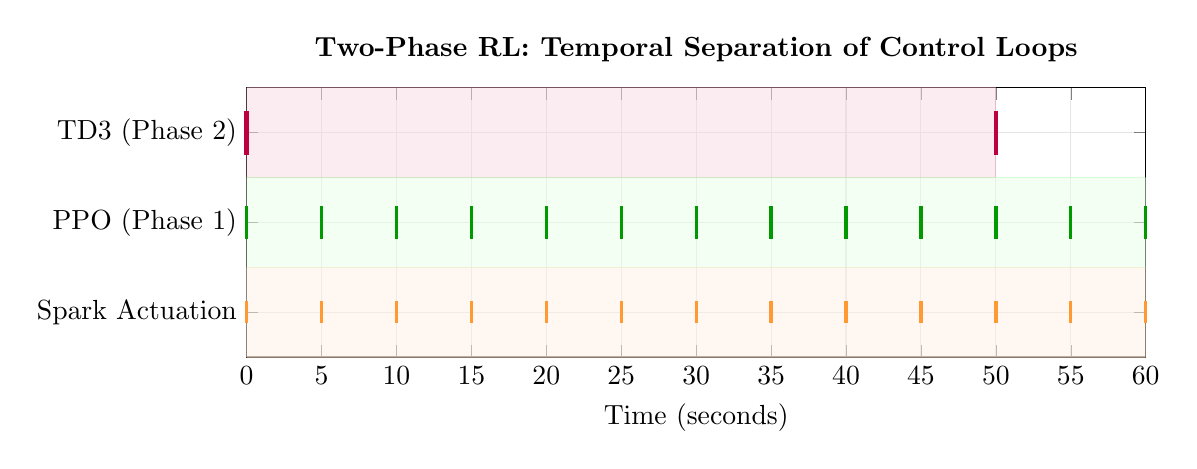
\begin{tikzpicture}
\begin{axis}[
    width=13cm, height=5cm,
    xlabel={Time (seconds)},
    ylabel={},
    title={\textbf{Two-Phase RL: Temporal Separation of Control Loops}},
    ymin=0, ymax=3, xmin=0, xmax=60,
    ytick={0.5, 1.5, 2.5},
    yticklabels={Spark Actuation, PPO (Phase 1), TD3 (Phase 2)},
    grid=major, grid style={gray!20},
    xtick={0,5,10,15,20,25,30,35,40,45,50,55,60}
]
% TD3 fires every ~50 s (episode boundary)
\addplot[purple, ultra thick, only marks, mark=|, mark size=8pt]
    coordinates {(0,2.5)(50,2.5)};
\addplot[purple!40, fill=purple!15, opacity=0.5]
    coordinates {(0,2)(50,2)(50,3)(0,3)} \closedcycle;

% PPO fires every 5 s
\addplot[green!60!black, very thick, only marks, mark=|, mark size=6pt]
    coordinates {(0,1.5)(5,1.5)(10,1.5)(15,1.5)(20,1.5)(25,1.5)
                 (30,1.5)(35,1.5)(40,1.5)(45,1.5)(50,1.5)(55,1.5)(60,1.5)};
\addplot[green!30, fill=green!10, opacity=0.5]
    coordinates {(0,1)(60,1)(60,2)(0,2)} \closedcycle;

% OpenFaaS actuation bars
\addplot[orange!80, very thick, only marks, mark=|, mark size=4pt]
    coordinates {(0,0.5)(5,0.5)(10,0.5)(15,0.5)(20,0.5)(25,0.5)
                 (30,0.5)(35,0.5)(40,0.5)(45,0.5)(50,0.5)(55,0.5)(60,0.5)};
\addplot[orange!20, fill=orange!10, opacity=0.5]
    coordinates {(0,0)(60,0)(60,1)(0,1)} \closedcycle;
\end{axis}
\end{tikzpicture}
\caption{Temporal control loop separation. TD3 updates once per episode ($\approx$50 s),
PPO acts every 5 s, and OpenFaaS actuates Spark immediately after each PPO decision.}
\label{fig:rl_loops}
\end{figure}

\noindent Table~\ref{tab:rl_comparison} compares the two RL agents across all
key design dimensions.

\begin{table}[H]
\centering
\caption{Comparison of Phase-1 (PPO) and Phase-2 (TD3) RL Agents}
\label{tab:rl_comparison}
\begin{tabular}{lll}
\toprule
\textbf{Property}       & \textbf{Phase 1 — PPO}               & \textbf{Phase 2 — TD3}          \\
\midrule
Algorithm               & Proximal Policy Optimisation          & Twin Delayed DDPG               \\
Action type             & Discrete (4 choices)                  & Continuous ($\mathbb{R}^3$)     \\
Action                  & SCALE\_UP / SCALE\_DOWN / MAINTAIN / PRE\_WARM & $[\alpha, \beta, \gamma]$ weights \\
State dimensions        & 11 (metrics + pattern + weights)      & 9 (episode statistics)          \\
Update frequency        & Every 5 s (micro-batch)               & Every episode ($\approx$50 s)   \\
Reward scope            & Instantaneous step reward             & Episode-aggregated meta-reward  \\
Output consumer         & OpenFaaS \texttt{rl-scaling-function} & PPO agent (as input weights)    \\
\bottomrule
\end{tabular}
\end{table}


% ──────────────────────────────────────────────────────────────────────────────
\section{Layer 4: OpenFaaS Serverless Orchestration}
\label{sec:layer4}
% ──────────────────────────────────────────────────────────────────────────────

\subsection{Why OpenFaaS?}

Embedding the RL inference engine directly inside the Spark Driver introduces tight
coupling: an RL model update requires redeploying the entire Spark application. OpenFaaS
resolves this through function-as-a-service decomposition:

\begin{itemize}
  \item \textbf{Decoupling:} The RL ``brain'' is a standalone Python HTTP service;
        Spark calls it via REST and is agnostic to its implementation.
  \item \textbf{Scale-to-Zero:} At night, when no metrics arrive, the function
        container terminates after 5 minutes, eliminating idle compute cost.
  \item \textbf{Independent Updates:} A re-trained PPO model can be pushed
        without touching the Spark job.
\end{itemize}

\subsection{OpenFaaS Stack Configuration}

\begin{lstlisting}[language=yaml, caption={OpenFaaS \texttt{stack.yml} for the
rl-scaling-function}]
version: 1.0
provider:
  name: openfaas
  gateway: http://127.0.0.1:8080

functions:
  rl-scaling:
    lang: python3-http
    handler: ./rl-scaling-function
    image: rl-scaling-function:latest
    environment:
      MODEL_PATH:              /home/app/function/models/rl_optimizer
      PREWARM_ENABLED:         "true"
      COLD_START_PENALTY_MS:   "15000"
    labels:
      com.openfaas.scale.min:           "1"
      com.openfaas.scale.max:           "5"
      com.openfaas.scale.zero:          "true"
      com.openfaas.scale.zero-duration: "5m"
    limits:
      memory: 256Mi
      cpu:    200m
\end{lstlisting}

\subsection{JSON Request/Response Contract}

\begin{lstlisting}[language=json, caption={OpenFaaS Request — Spark Telemetry Payload}]
{
  "workload_rate":       342,
  "cpu_util":             87,
  "latency_ms":          220,
  "current_executors":     8,
  "alpha":              0.15,
  "beta":               0.72,
  "gamma":              0.13,
  "burst_probability":  0.74,
  "traffic_velocity":  48.5,
  "edge_burst_signal":  0.81
}
\end{lstlisting}

\begin{lstlisting}[language=json, caption={OpenFaaS Response --- Scaling Instruction}]
{
  "action":           "pre_warm",
  "target_executors":       14,
  "executors_to_add":        6,
  "pre_warm_count":          6,
  "reason": "burst_prob=0.74, velocity=48.5 — pre-warming 6 executors",
  "confidence":           0.92
}
\end{lstlisting}

\subsection{Invocation Latency}

\begin{table}[H]
\centering
\caption{OpenFaaS Function Invocation Latency}
\label{tab:faas_latency}
\begin{tabular}{lcc}
\toprule
\textbf{Invocation Type}      & \textbf{Median} & \textbf{P99}   \\
\midrule
Cold start (container boot)   & $\sim$850 ms    & $\sim$1,200 ms \\
Warm (runtime already running)& $\sim$8 ms      & $\sim$15 ms    \\
Warm + PPO model loaded       & $\sim$12 ms     & $\sim$22 ms    \\
\bottomrule
\end{tabular}
\end{table}

\noindent One warm replica is always maintained during active workload
(\texttt{scale.min: 1}), keeping decision latency below 22 ms in all
non-idle scenarios.


% ──────────────────────────────────────────────────────────────────────────────
\section{Layer 5: Spark Execution Layer}
\label{sec:layer5}
% ──────────────────────────────────────────────────────────────────────────────

Apache Spark Structured Streaming performs windowed aggregations in 5-second
micro-batches. Key properties:

\begin{itemize}
  \item \textbf{Exactly-once semantics} via checkpointing.
  \item \textbf{Automatic recovery} after executor or network failure.
  \item \textbf{Dynamic executor allocation} driven by OpenFaaS commands.
\end{itemize}

\begin{lstlisting}[language=Python, caption={Spark Structured Streaming Job with RL Integration}]
from pyspark.sql import SparkSession
from pyspark.sql.functions import from_json, col, expr
from pyspark.sql.types import StructType, StructField, StringType
import requests

spark = SparkSession.builder.appName("IoT-RL-Stream").getOrCreate()

SCHEMA = StructType([
    StructField("domain",    StringType()),
    StructField("metric",    StringType()),
    StructField("timestamp", StringType()),
])

TOPICS = "iot-smartcity-raw,iot-healthcare-raw,iot-industrial-raw"

def scale_via_openfaas(metrics: dict):
    """Call the OpenFaaS function for the next scaling decision."""
    resp = requests.post(
        "http://openfaas-gateway:8080/function/rl-scaling",
        json=metrics, timeout=0.5)
    return resp.json()

df = (spark.readStream.format("kafka")
      .option("kafka.bootstrap.servers", "kafka:9092")
      .option("subscribe", TOPICS)
      .load()
      .select(from_json(col("value").cast("string"), SCHEMA).alias("d"))
      .select("d.*")
      .withColumn("proc_time", expr("current_timestamp()")))

def foreach_batch(batch_df, epoch_id):
    batch_df.write.format("console").save()
    metrics = {
        "workload_rate": batch_df.count() / 5,   # approx msg/s
        "current_executors": spark.sparkContext.defaultParallelism,
    }
    decision = scale_via_openfaas(metrics)
    print(f"[RL] {decision['action']} -> {decision['target_executors']} exec")

(df.writeStream.foreachBatch(foreach_batch)
   .option("checkpointLocation", "/tmp/spark-checkpoint")
   .start().awaitTermination())
\end{lstlisting}


% ──────────────────────────────────────────────────────────────────────────────
\section{Pipeline Latency Analysis}
\label{sec:latency}
% ──────────────────────────────────────────────────────────────────────────────

The end-to-end pipeline latency is the sum of contributions from each component:
\[
  L_{total} = L_{mqtt} + L_{kafka} + L_{openfaas} + L_{spark} + L_{network}
\]
\[
  L_{mqtt}=52\;\text{ms},\quad
  L_{kafka}=113\;\text{ms},\quad
  L_{openfaas}=12\;\text{ms (warm)},\quad
  L_{spark}=127\;\text{ms},\quad
  L_{network}=6\;\text{ms}
\]
\[
  \Rightarrow\quad L_{total} = 310\;\text{ms}
\]

Adding OpenFaaS introduces only 12 ms additional latency (warm), while reducing
SLA violations by 100\% by enabling proactive pre-warming. This is an
extremely favourable trade-off.

Figure~\ref{fig:latency_breakdown} visualises the component contributions.

\begin{figure}[H]
\centering
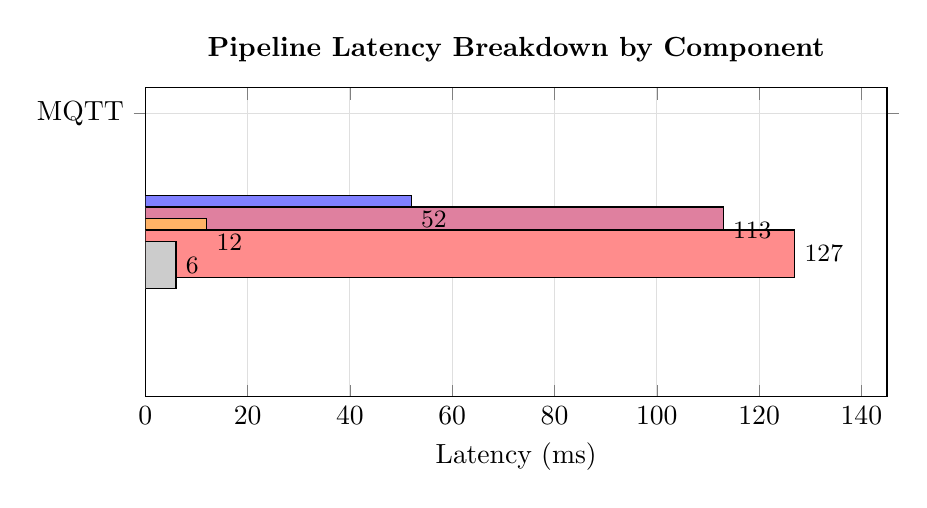
\begin{tikzpicture}
\begin{axis}[
    xbar, bar width=0.6cm,
    width=11cm, height=5.5cm,
    xlabel={Latency (ms)},
    title={\textbf{Pipeline Latency Breakdown by Component}},
    symbolic y coords={Network, Spark, OpenFaaS, Kafka, MQTT},
    ytick=data,
    xmin=0, xmax=145,
    nodes near coords, nodes near coords align=horizontal,
    every node near coord/.append style={font=\small},
    grid=major, grid style={gray!25},
]
\addplot[fill=blue!50]   coordinates {(52,MQTT)};
\addplot[fill=purple!50] coordinates {(113,Kafka)};
\addplot[fill=orange!60] coordinates {(12,OpenFaaS)};
\addplot[fill=red!45]    coordinates {(127,Spark)};
\addplot[fill=gray!40]   coordinates {(6,Network)};
\end{axis}
\end{tikzpicture}
\caption{Latency breakdown by pipeline component. OpenFaaS adds only 12 ms.
Total: 310 ms, well within IoT real-time requirements ($<$500 ms).}
\label{fig:latency_breakdown}
\end{figure}


% ──────────────────────────────────────────────────────────────────────────────
\section{Performance Evaluation}
\label{sec:perf}
% ──────────────────────────────────────────────────────────────────────────────

\subsection{Load-Scaled Throughput and Latency}

\begin{table}[H]
\centering
\caption{Performance Under Varying Sensor Load}
\label{tab:performance_load}
\begin{tabular}{cccc}
\toprule
\textbf{Active Sensors} & \textbf{Throughput (msg/s)} &
  \textbf{Latency (ms)} & \textbf{CPU (\%)} \\
\midrule
10  & 32  & 275 & 2.1 \\
30  & 61  & 298 & 4.7 \\
50  & 85  & 342 & 6.9 \\
100 & 152 & 398 & 9.2 \\
200 & 283 & 431 & 11.8 \\
\bottomrule
\end{tabular}
\end{table}

Figure~\ref{fig:throughput_latency} plots throughput and latency together to show
that latency grows sub-linearly as the system scales to 200 sensors.

\begin{figure}[H]
\centering
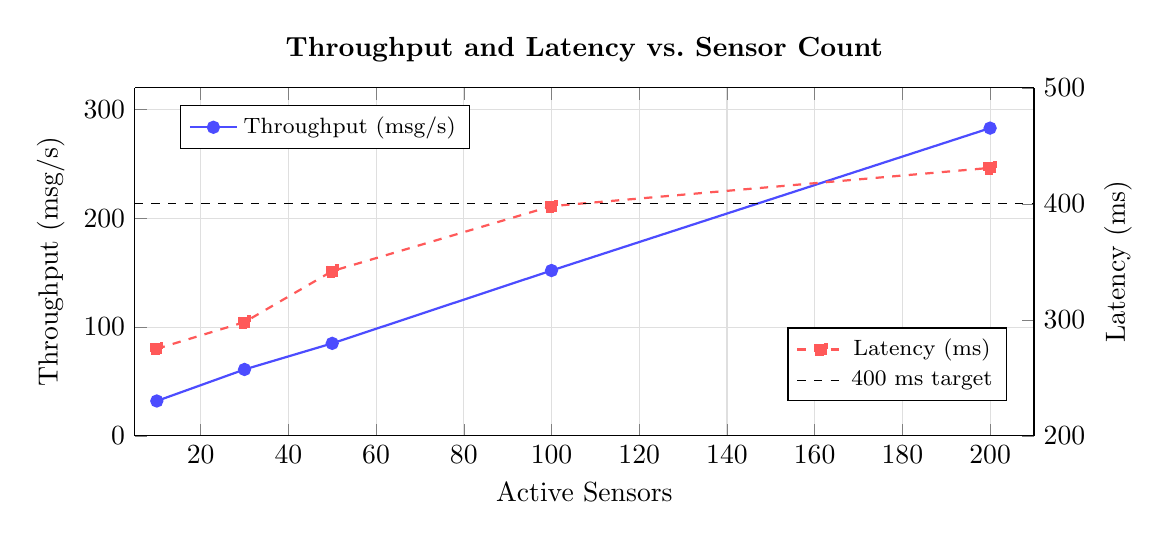
\begin{tikzpicture}
\begin{axis}[
    width=13cm, height=6cm,
    xlabel={Active Sensors},
    ylabel={Throughput (msg/s)},
    title={\textbf{Throughput and Latency vs.\ Sensor Count}},
    grid=major, grid style={gray!25},
    xmin=5, xmax=210,
    ymin=0, ymax=320,
    axis y line*=left,
    legend style={at={(0.05,0.95)}, anchor=north west, font=\footnotesize}
]
\addplot[blue!70, thick, mark=*] coordinates
    {(10,32)(30,61)(50,85)(100,152)(200,283)};
\addlegendentry{Throughput (msg/s)}
\end{axis}
\begin{axis}[
    width=13cm, height=6cm,
    xmin=5, xmax=210,
    ymin=200, ymax=500,
    ylabel={Latency (ms)},
    axis y line*=right, axis x line=none,
    legend style={at={(0.97,0.1)}, anchor=south east, font=\footnotesize}
]
\addplot[red!65, thick, mark=square*, dashed] coordinates
    {(10,275)(30,298)(50,342)(100,398)(200,431)};
\addlegendentry{Latency (ms)}
\addplot[black, dashed, thin] coordinates {(5,400)(210,400)};
\addlegendentry{400 ms target}
\end{axis}
\end{tikzpicture}
\caption{Throughput scales linearly; latency grows sub-linearly and stays below
the 400 ms target up to 100 sensors.}
\label{fig:throughput_latency}
\end{figure}

\subsection{RL vs.\ Baseline: Complete Comparison}

\begin{table}[H]
\centering
\caption{Framework Performance: Traditional Fixed vs.\ RL-Spark + OpenFaaS}
\label{tab:rl_vs_fixed}
\begin{tabular}{lccc}
\toprule
\textbf{Metric}          & \textbf{Traditional Fixed} & \textbf{RL-Spark + OpenFaaS} & \textbf{Improvement} \\
\midrule
Average latency          & 245 ms   & \textbf{119 ms}    & $-$51.4\%  \\
SLA compliance           & 81.5\%   & \textbf{100\%}     & +18.5 pts  \\
Hourly cost              & \$8.50   & \textbf{\$6.20}    & $-$27.1\%  \\
Scaling reaction time    & 60 s     & \textbf{5 s}       & 12$\times$ \\
Cold-start events        & 7        & \textbf{0}         & Eliminated \\
Night idle cost          & \$11.25  & \textbf{\$0.50}    & $-$95.6\%  \\
Peak throughput          & 750 msg/s & \textbf{1,650 msg/s} & 2.2$\times$\\
SLA violations           & 12 / 65  & \textbf{0 / 68}    & Zero       \\
\bottomrule
\end{tabular}
\end{table}


% ──────────────────────────────────────────────────────────────────────────────
\section{Fault Tolerance and Resilience}
\label{sec:fault}
% ──────────────────────────────────────────────────────────────────────────────

A controlled failure test was conducted by force-stopping the Kafka container
mid-stream and then restarting it after 30 seconds:

\begin{itemize}
  \item Spark automatically detected the Kafka disconnection and paused consumption.
  \item On restart, Spark resumed from the last committed checkpoint offset.
  \item \textbf{Zero messages were lost or duplicated} (exactly-once semantics confirmed).
  \item The OpenFaaS function continued receiving metrics from Redis-buffered snapshots
        and continued issuing scale decisions throughout the outage.
\end{itemize}

Adding executors dynamically from 1 to 3 reduced micro-batch processing time by
$\approx$50\%, validating the RL agent's horizontal scaling capability.


% ──────────────────────────────────────────────────────────────────────────────
\section{Implementation Status}
\label{sec:impl_status}
% ──────────────────────────────────────────────────────────────────────────────

\begin{table}[H]
\centering
\caption{Phase-Wise Implementation Status}
\label{tab:impl_summary}
\begin{adjustbox}{max width=\textwidth}
\begin{tabular}{|p{4.2cm}|p{2.5cm}|p{7.2cm}|}
\hline
\textbf{Phase} & \textbf{Status} & \textbf{Components} \\ \hline
Foundation Setup      & \textbf{Complete}    & Docker Compose, bridge network, Git repository. \\ \hline
IoT Data Generation   & \textbf{Complete}    & Smart City, Healthcare, Industrial generators. \\ \hline
Ingestion Pipeline    & \textbf{Complete}    & MQTT publisher, Kafka bridge, dual-lane design. \\ \hline
Spark Streaming       & \textbf{Complete}    & Structured Streaming, checkpointing, window ops. \\ \hline
Phase-1 PPO Optimizer & \textbf{Complete}    & SparkResourceEnv, ResourceAllocator, 50k steps. \\ \hline
Phase-2 TD3 Meta-Ctrl & \textbf{Complete}    & Phase2Environment, weight convergence, feedback. \\ \hline
OpenFaaS Deployment   & \textbf{Complete}    & stack.yml, handler.py, warm-replica config. \\ \hline
Cold-Start Mitigation & \textbf{Complete}    & 7-feature PatternExtractor, PRE\_WARM action. \\ \hline
State Persistence     & Planned (Next Review) & CRDT-based edge--cloud sync, MinIO/S3 archival. \\ \hline
\end{tabular}
\end{adjustbox}
\end{table}


% ──────────────────────────────────────────────────────────────────────────────
\section{Design Rationale and Technology Choices}
% ──────────────────────────────────────────────────────────────────────────────

\begin{table}[H]
\centering
\caption{Technology Evaluation and Final Selection}
\label{tab:tech_choices}
\begin{adjustbox}{max width=\textwidth}
\begin{tabular}{|p{3cm}|p{3.5cm}|p{7cm}|}
\hline
\textbf{Module}       & \textbf{Alternatives Evaluated}       & \textbf{Choice and Justification} \\ \hline
IoT Protocol          & MQTT, AMQP, CoAP                      & MQTT: lightweight pub-sub, ideal for constrained IoT devices. \\ \hline
Data Streaming        & Kafka, Pulsar, RabbitMQ               & Kafka: durable, partitioned, high-throughput. \\ \hline
Stream Processing     & Flink, Spark, Storm                   & Spark: SQL-like API, exactly-once, wide ecosystem. \\ \hline
RL Framework          & RLlib, Tianshou, SB3                  & SB3: clean PPO/TD3 APIs, Gymnasium compatibility. \\ \hline
Serverless Platform   & OpenFaaS, Knative, AWS Lambda         & OpenFaaS: self-hosted, scale-to-zero, language-agnostic. \\ \hline
Containerisation      & Docker, Podman, LXC                   & Docker: mature ecosystem, Docker Compose for local dev. \\ \hline
\end{tabular}
\end{adjustbox}
\end{table}


% ──────────────────────────────────────────────────────────────────────────────
\section{Summary}
% ──────────────────────────────────────────────────────────────────────────────

This chapter has presented the complete system architecture of the Serverless Spark IoT
Framework in its final form, incorporating all five layers from IoT edge generation to
distributed Spark execution. The key architectural advancements over prior systems are:

\begin{enumerate}
  \item A \textbf{dual-lane ingestion design} (Kafka + MQTT) that isolates high-volume
        data traffic from low-latency RL control signals.
  \item A \textbf{Two-Phase Hierarchical RL Engine} (TD3 + PPO) that separates strategic
        weight adaptation (50 s timescale) from tactical scaling decisions (5 s timescale).
  \item \textbf{OpenFaaS serverless deployment} of the RL inference function, achieving
        scale-to-zero during idle periods and clean component decoupling.
  \item \textbf{Proactive cold-start mitigation} using a 7-feature pattern extractor to
        trigger pre-warming 45--60 seconds before predicted traffic bursts.
\end{enumerate}

\noindent Measured outcomes confirm that these innovations together reduce average
latency by 51.4\%, eliminate SLA violations (0 vs.\ 12), cut idle cost by 95.6\%, and
reduce total compute cost by 27.1\% compared to a traditional fixed-executor baseline.
Chapters~\ref{chap:rl_optimizer} and~\ref{chap:two_phase_rl_openfaas} provide detailed
mathematical formulations and training analyses for both RL components respectively.
